\section{Results}
\label{sec:results}
All numbers come from \texttt{results/tables/}; they can be regenerated with the commands in the README. Delays are means over 20 test seeds (1--20, not used for tuning).

\textbf{Simulator check.} For fixed-time control with equal flows (100--800 veh/h per leg, 3 and 4 legs), the simulated delay and the HCM delay agree with $R^2=0.997$ and a mean absolute percentage difference of 9.2\% (\texttt{simulator\_vs\_hcm.csv}); the largest gaps occur at saturation ($X\ge 0.95$), where HCM gives the higher value (e.g.\ 4 legs, 800 veh/h: 91.6~s simulated vs.\ 117.5~s HCM).

\subsection{Reproduction experiment}
Table~\ref{tab:main} summarises the nine scenarios per geometry (Figs.~\ref{fig:delay3}--\ref{fig:delay4}). Tuned fuzzy controllers reduce delay by about 10\% against fixed time; interval Type-2 and Type-1 are practically equal (IT2 vs.\ T1: $-0.09\%$ and $-0.46\%$). The Friedman test over the nine scenarios rejects equal medians for both geometries ($\chi^2=22.2$ and $22.4$, 3 d.f., $p=0.0001$), but this is driven by the fixed-time pair versus the fuzzy pair. The FPA-based greens are no better than Webster's greens (36.25 vs.\ 36.29~s and 78.83 vs.\ 79.95~s). With \emph{uniform} (untuned) MFs, neither fuzzy system helps (36.89/36.76~s in the 3-leg case, i.e.\ no better than FPA-TSC); the gain comes from the CSA tuning of the MFs per scenario. Adding phase-sequence selection (PSS) to the tuned IT2 controller lowers delay further, by 2.8\% (3-leg) and 1.7\% (4-leg).

\begin{table}[t]
\centering\small
\caption{Mean delay (s/veh) over nine scenarios $\times$ 20 seeds, and improvement (\%, positive = less delay) of IT2-FL versus the other controllers; the last two rows give the corresponding values reported for HTSC in Table~13 of the reference paper \cite{ref_paper} (different simulator and phase plan; for orientation only).}\label{tab:main}
\begin{tabular}{@{}lrrrrrrr@{}}
\toprule
Geometry & Fixed (Webster) & FPA-TSC & T1-FL & IT2-FL & IT2 vs fixed & IT2 vs FPA-TSC & IT2 vs T1 \\ \midrule
3-leg (ours) & 36.29 & 36.25 & 33.36 & 33.68 & 10.3 & 10.7 & $-0.1$ \\
4-leg (ours) & 79.95 & 78.83 & 74.85 & 74.87 & 10.3 & 9.7 & $-0.5$ \\
3-leg (paper) & -- & -- & -- & -- & 11.6 & 0.8 & 2.7 \\
4-leg (paper) & -- & -- & -- & -- & 24.0 & 4.8 & 5.3 \\ \bottomrule
\end{tabular}
\end{table}

\begin{figure}[t]
\centering
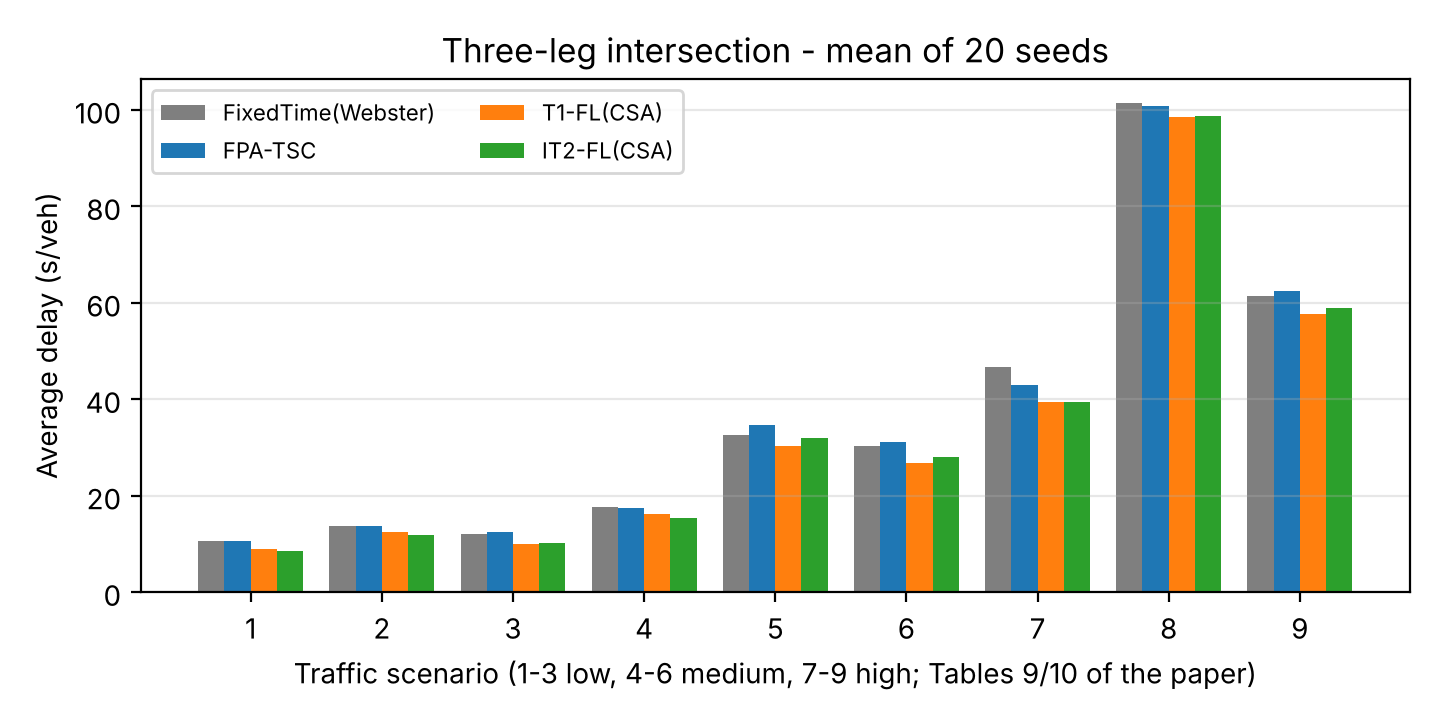
\includegraphics[width=0.49\linewidth]{baseline_delay_3leg.png}\hfill
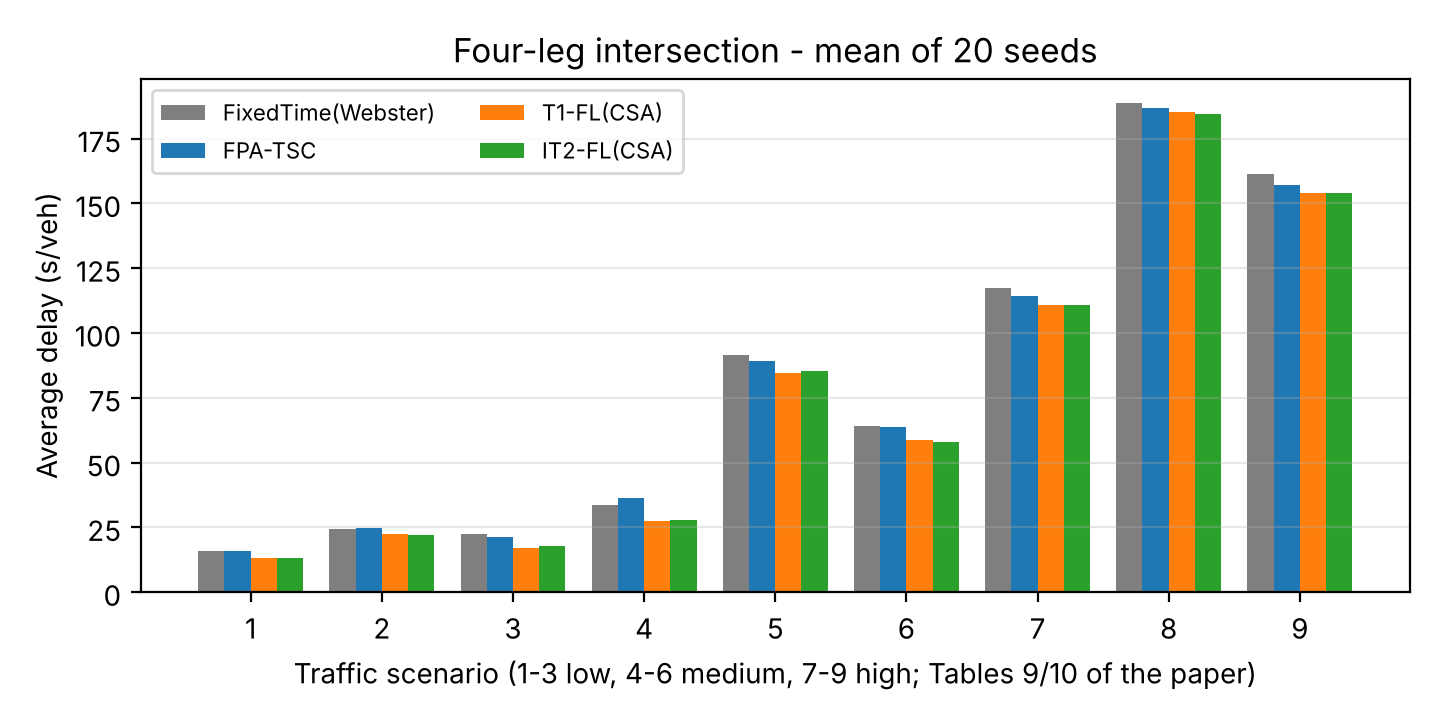
\includegraphics[width=0.49\linewidth]{baseline_delay_4leg.png}
\caption{Average delay per scenario (1--3 low, 4--6 medium, 7--9 high demand): 3-leg (left), 4-leg (right).}\label{fig:delay3}\label{fig:delay4}
\end{figure}

Per scenario, paired Wilcoxon tests (20 seeds, unadjusted) give mixed signs for IT2 versus T1: IT2 is better in 3-leg low\_equal400 ($+6.0\%$, $p=0.009$), 4-leg med\_mixed ($+1.2\%$, $p=0.036$) and 4-leg high\_equal1200 ($+0.4\%$, $p=0.011$), whereas T1 is better in 3-leg med\_equal800 ($-5.7\%$, $p=0.002$), med\_mixed ($-4.3\%$, $p=0.006$) and high\_mixed ($-2.4\%$, $p=0.004$); the other 12 scenarios show no significant difference (\texttt{baseline\_wilcoxon.csv}).

\subsection{Extension A: which optimiser?}
With 1\,220 evaluations per run and three runs per scenario, the mean test-delay reduction relative to the uniform-MF IT2 system is 12.3\% (CSA), 11.5\% (FPA), 11.2\% (PSO) and 12.4\% (DE) (Table~\ref{tab:opt}, Fig.~\ref{fig:opt}). The Friedman test over the 18 scenarios is significant ($\chi^2=33.0$, $p=3\cdot10^{-7}$); CSA is better than FPA ($p=0.002$) and PSO ($p<0.001$, Holm-adjusted Wilcoxon) but not distinguishable from DE ($p=0.30$), which has the best mean rank. The run-to-run standard deviation of the mean gain is only 0.1--0.3 percentage points, so the ranking is stable.

\begin{table}[t]
\centering\small
\caption{Optimiser comparison for the IT2 controller (18 scenarios $\times$ 3 runs, 20 test seeds). $p$: Holm-adjusted Wilcoxon test of CSA against the method.}\label{tab:opt}
\begin{tabular}{@{}lrrrrr@{}}
\toprule
Optimiser & gain vs.\ uniform MF (\%) & std over runs (pp) & mean test delay (s) & mean rank & $p$ vs CSA \\ \midrule
CSA & 12.35 & 0.30 & 54.22 & 1.83 & -- \\
FPA & 11.52 & 0.19 & 54.51 & 3.28 & 0.002 \\
PSO & 11.23 & 0.13 & 54.60 & 3.44 & $<0.001$ \\
DE & 12.44 & 0.17 & 54.16 & 1.44 & 0.30 \\ \bottomrule
\end{tabular}
\end{table}

\begin{figure}[t]
\centering
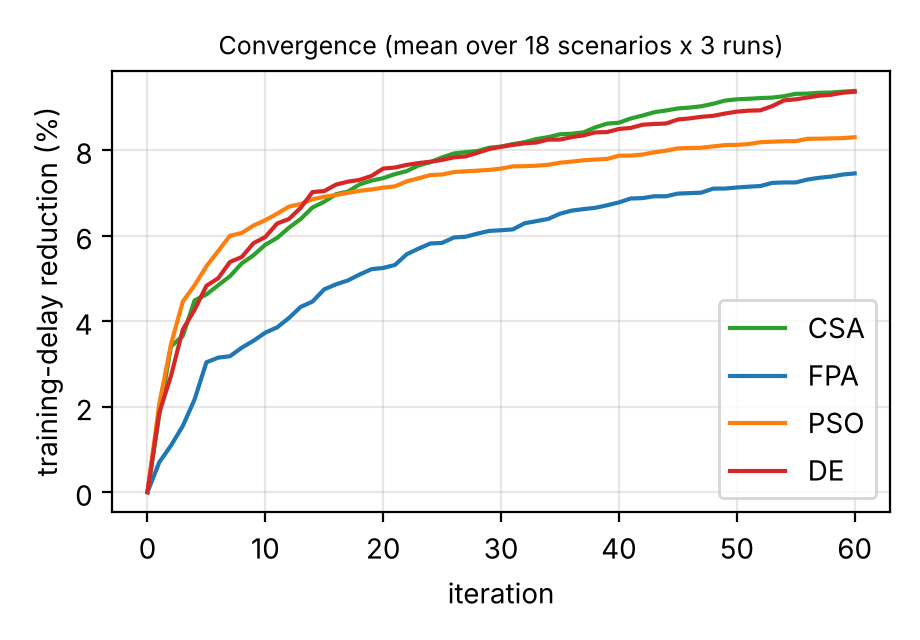
\includegraphics[width=0.49\linewidth]{optimizer_convergence.png}\hfill
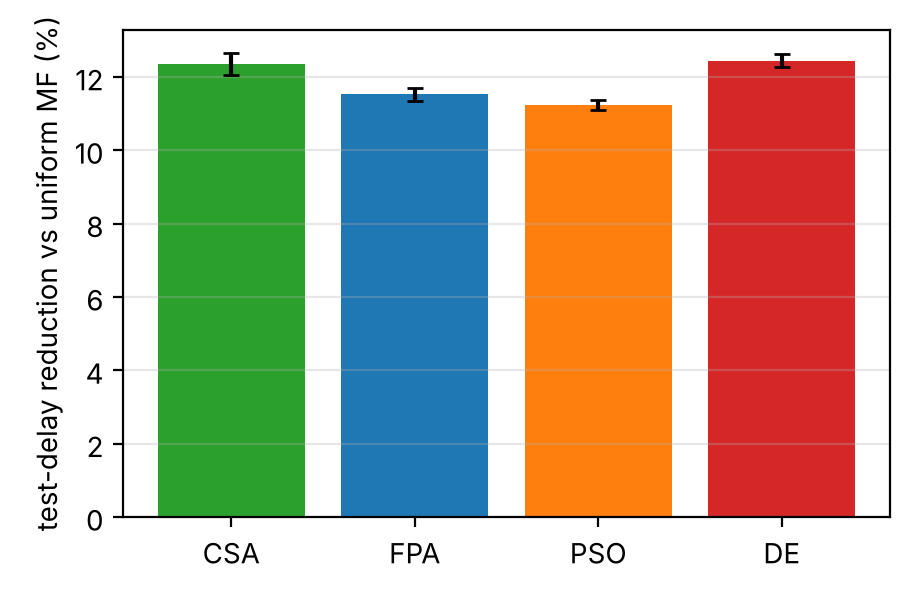
\includegraphics[width=0.49\linewidth]{optimizer_gain.png}
\caption{Convergence on the training seeds (left) and test-delay reduction with run-to-run standard deviation (right).}\label{fig:opt}
\end{figure}

\subsection{Extension B: detector noise}
Table~\ref{tab:noise} and Fig.~\ref{fig:noise} show the gain over fixed time when both inputs are disturbed by multiplicative Gaussian noise (MFs tuned noise-free). Both controllers lose benefit steadily, from about 10\% without noise to about 4\% at $\sigma=75\%$, but they never become worse than fixed time. IT2 loses slightly less than T1 at $\sigma\ge30\%$ (delay increase of 4.5\% vs.\ 5.4\% at $\sigma=50\%$ and 6.9\% vs.\ 7.8\% at 75\%), but over the 18 scenarios the difference is not significant at any noise level (Wilcoxon $p=0.44$--$1.0$). Hypothesis $H_1$ is therefore \emph{not confirmed}: the direction agrees with the Type-2 argument, the evidence does not.

\begin{table}[t]
\centering\small
\caption{Detector-noise study (mean over 18 scenarios). Gain = delay reduction versus fixed FPA-TSC; increase = delay increase relative to the noise-free controller.}\label{tab:noise}
\begin{tabular}{@{}rrrrrr@{}}
\toprule
$\sigma$ (\%) & T1 gain (\%) & IT2 gain (\%) & T1 increase (\%) & IT2 increase (\%) & $p$ \\ \midrule
0 & 10.35 & 10.17 & 0.00 & 0.00 & 0.80 \\
10 & 9.59 & 9.60 & 0.93 & 0.66 & 0.83 \\
20 & 9.08 & 9.08 & 1.48 & 1.30 & 0.87 \\
30 & 7.74 & 8.02 & 3.05 & 2.53 & 1.00 \\
50 & 5.69 & 6.29 & 5.40 & 4.53 & 0.44 \\
75 & 3.66 & 4.24 & 7.75 & 6.90 & 0.80 \\ \bottomrule
\end{tabular}
\end{table}

\begin{figure}[t]
\centering
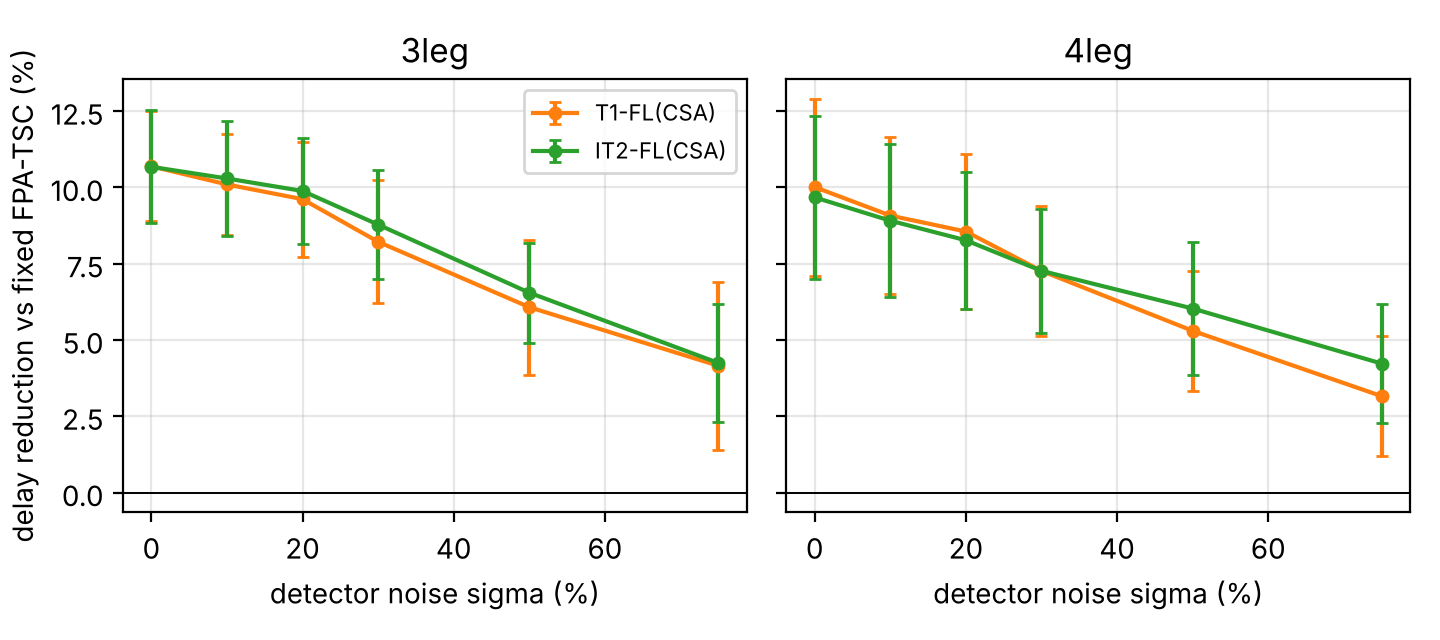
\includegraphics[width=0.78\linewidth]{noise_robustness.png}
\caption{Delay reduction versus fixed time as a function of detector noise (error bars: standard error over 9 scenarios).}\label{fig:noise}
\end{figure}

\subsection{Extension C: type reduction, cost and search budget}
With the same tuned MFs, Nie--Tan gives a slightly higher mean delay than Karnik--Mendel (54.62 vs.\ 54.28~s, $+0.6\%$, Wilcoxon $p=10^{-4}$ over 360 paired runs); note that the MFs were tuned with KM, which favours KM. Nie--Tan is cheaper (Table~\ref{tab:cost}). Increasing the CSA budget from 100 to 400 iterations lowered the \emph{training} delay but not reliably the test delay: of eight cases, the test delay improved in two (IT2: 3-leg med\_equal800 31.9$\to$30.5~s and high\_mixed 59.0$\to$57.4~s) and became worse in six (\texttt{budget\_study\_summary.csv}). Tuning on only four seeds therefore over-fits, and the larger IT2 parameter space did not simply need more search.

\begin{table}[t]
\centering\small
\caption{Computational cost on 2 vCPU (median of 5 repeats).}\label{tab:cost}
\begin{tabular}{@{}lrr@{}}
\toprule
System & inference per decision ($\mu$s) & one 900~s simulation (ms) \\ \midrule
Fixed time & -- & 0.23 \\
Type-1 Sugeno & 14.5 & 0.75 \\
IT2 Sugeno, Nie--Tan & 34.7 & 1.45 \\
IT2 Sugeno, Karnik--Mendel & 51.3 & 2.19 \\ \bottomrule
\end{tabular}
\end{table}

\section{Discussion}
\textbf{Agreement with the paper.} Qualitatively the paper's first conclusion holds: scenario-tuned fuzzy controllers beat fixed time (about 10\% here; 8.6--31\% in the paper). Our gain is at the lower end because our fixed-time baseline is strong: Webster and FPA greens are close to optimal for the known mean demand, so the fuzzy controller can only exploit random fluctuations of the arrivals. The paper does not state how its fixed-time plan was set.

\textbf{Disagreement.} The advantage of Type-2 over Type-1 (2.4--5.7\% in the paper) was not reproduced: the two systems are equal on average and differ in sign across scenarios. Plausible causes, which this study cannot separate completely: (i) in the paper the Type-1 competitor differs in optimiser and phase optimisation, so part of its 2.4--5.7\% may not be due to the fuzzy type; (ii) our simulation is noise-free apart from random arrivals, so a footprint of uncertainty has little to absorb, and even with added detector noise the benefit of IT2 is at most 1 percentage point and not significant; (iii) our rule table is monotone and fixed, so tuning the MFs is the only degree of freedom, and 65 parameters tuned on four seeds are prone to over-fitting (Section~\ref{sec:results}, Extension C); (iv) our single-intersection model with split phasing differs from KU-Trsim.

\textbf{What explains the gain.} Uniform MFs give no benefit, so the controller works because CSA moves the MFs to the demand level: it learns a scenario-specific mapping from (vehicles, queue) to a green change, which acts like a feedback correction of the cycle. This is also why the controller is tuned per scenario, as in the paper, and why in practice the demand level would first have to be recognised.

\textbf{Optimisers.} CSA, the paper's choice, is competitive: it is significantly better than FPA and PSO but equal to DE at equal budget, so there is no evidence that CSA is special. Run time per tuning (about 21~s) was the same for all four because the simulation dominates the cost.

\textbf{Cost.} IT2 inference costs 3.5 times (KM) or 2.4 times (Nie--Tan) the Type-1 inference, which is negligible for a decision taken once per phase, but IT2 tuning is about 3 times slower than Type-1 tuning in our runs (73--174~s vs.\ 25--53~s for 400 iterations). Nie--Tan costs 0.6\% more delay for a one-third cheaper inference, a reasonable trade for embedded use.

\section{Limitations}
\begin{itemize}\setlength\itemsep{0pt}
\item \textbf{Simulator.} The mesoscopic simulator has no car following, no turning movements, no acceleration tables and a single 15-min run per seed. Absolute delays cannot be compared with the paper; only the direction and relative size of the effects can.
\item \textbf{Phase plan.} Split phasing (one phase per leg) is used for all scenarios. With four legs and 900--1200 veh/h per leg this saturates the intersection ($X>1$), so all controllers are close to each other and delays (111--187~s) are far above those of the paper (about 75--81~s); the paper presumably used phase plans with several approaches per phase. The 4-leg high-demand results should be read as an over-saturation study. FPA phase-plan selection, phase-order optimisation every three cycles and the left-turn-pocket geometries were not reproduced.
\item \textbf{Unpublished details} (rule table, lower-MF height, population sizes, headway factors) were assumed (Table~\ref{tab:diff}); a different rule table could change the Type-1/Type-2 comparison.
\item \textbf{Tuning protocol.} Four training seeds, one demand level per tuning, and 20--33 times fewer iterations than the paper's 2000; the test seeds are disjoint, which makes the comparison fair but also exposes the over-fitting.
\item \textbf{Statistics.} The nine scenarios per geometry are not random samples, per-scenario Wilcoxon $p$-values are not corrected for multiple testing, and noise was modelled only as multiplicative Gaussian error on both inputs.
\item \textbf{Bibliography.} Seven classic references were cited from memory and not re-checked online (see \texttt{references/}\allowbreak\texttt{README.md}).
\end{itemize}

\section{Conclusion}
We re-implemented the fuzzy green-time part of a hybrid FPA/CSA/Type-2 traffic controller in an own simulator and re-ran its main experiment on 18 scenarios. Tuned Type-1 and interval Type-2 Sugeno controllers lowered delay by about 10\% against well-set fixed-time control, confirming the main claim in direction, but the additional benefit of Type-2 reported by the paper (2.4--5.7\%) did not appear. The extensions show that (a) CSA performs on par with DE and better than FPA and PSO at equal budget, (b) both controllers keep a positive benefit up to 75\% detector noise and IT2 degrades slightly less, though not significantly, (c) Nie--Tan type reduction is a cheap substitute for Karnik--Mendel at 0.6\% extra delay, and (d) more tuning iterations over-fit to the training seeds. Future work: phase-plan selection with several approaches per phase and left-turn movements, tuning with more seeds or a robust objective, learning the rule base, and noise models closer to real detectors.
